\section{Evaluation of Environmental Wireless Sensor Networks (E-WSN)}
\label{section:experimental}	

The simulation framework to evaluate the algorithms' performance was based on a realistic deployment scenario as covered by  \cite{Gomez2015} and others \cite{Jha2016, Avram}. In this scenario a UAV is used to deploy a large number of sensors over a expansive and remote geographical area, giving an ad-hoc, randomised placement of devices. Solar power cells are used to maintain enough energy to power the sensors over a number of years, given low enough power consumption. We make the following assumptions and simplifications.
\begin{itemize}{
		\item Node deployment is randomly distributed across the grid following the uniform distribution or a radial normal distribution.
		\item Energy harvesting works continuously at constant rate. This assumes consistent solar exposure and limits the simulation to daytime.
		\item Permanent node failure is based on the total energy consumption of that node over time, as a proxy for wear.
		\item Temporary loss of availability of nodes is random and at a constant rate.
	}
\end{itemize}
Example values in \ref{table:components_energy_usage} show the energy and time costs of varios operations given an hourly sampling period for a node.
\begin{table}[ht]
	\begin{tabular}{p{0.3\textwidth}p{0.2\textwidth} p{0.2\textwidth} p{0.2\textwidth}}
		\hline
		\textbf{Function} & \textbf{power(mW)} & \textbf{time (s)} & \textbf{energy (mJ)}\\
		\hline
		Data acquisition (\symbolDataAcquisition{}{}) & 0.5 & 60 & 30 \\
		Transmission (\symbolTransmission{}{}) & 7 & 0.1 & 0.7 \\
		Receiver (\symbolReceiver{}{}) & 70 & 0.1 & 0.7 \\
		Idle wake-up-radio (\symbolWakeUpRadio{}{}) & 0.07 & 3509 & 246  \\
		\hline
	\end{tabular}
	\caption{Component types and energy usage}
	\label{table:components_energy_usage}
\end{table}

\todo[inline]{Describe the comparison of network task layouts}
\begin{figure}[ht]
	\centering
	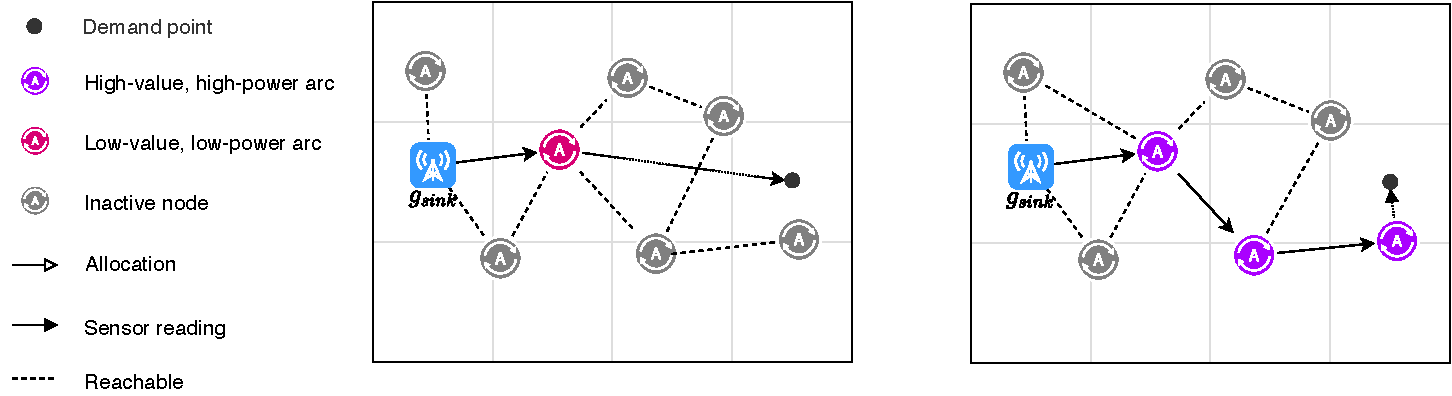
\includegraphics[width=0.9\linewidth]{route-types}
	\caption{\textbf{Routes, power consumption, and task value}. The diagram shows two possible arcs possible for the same system. In the first, energy is conserved by having a short arc but the task is completed to a lesser quality. In the second, the maximum quality for the task is achieved, however, there is more energy consumption overall.}
	\label{fig:route_types}
\end{figure}

